\documentclass[a4paper,oneside]{Tptesi2}

\usepackage[italian]{babel}
\usepackage{listings}
\usepackage{amsmath,amssymb}
\usepackage{verbatim}
\usepackage{indentfirst}
\usepackage[utf8]{inputenc}
\usepackage{subfigure}
\usepackage{algorithmic}
\usepackage{framed}
\usepackage{rotating}
\usepackage{cite}
\usepackage{graphicx}
\usepackage[]{algorithm2e}
\usepackage[font=small,labelfont=bf]{caption}




% Packages -----------------------------------------------------------------------
%\usepackage{amsthm}
%\usepackage{amsmath}          % Non necessario se usi TPTESI2 perche' gia` incluso
%\usepackage[dvips]{graphicx}  % Non necessario se usi TPTESI2 perche' gia` incluso
%\usepackage{url} %non usare se si usa hyperref


\newcommand{\mr}{\emph{motore di ricerca}}
\newcommand{\Mr}{\emph{Motore di ricerca}}
\newcommand{\ws}{Web~service }


% Use a small font for the verbatim environment
\makeatletter  % makes '@' an ordinary character
\renewcommand{\verbatim@font}{%
  \ttfamily\footnotesize\catcode`\<=\active\catcode`\>=\active%
}
\makeatother   % makes '@' a special symbol again
%
% Simboli Matematici -------------------------------------------------------------
%\newcommand{\h}{\mathcal{H}_\infty} % scorciatoia per sequenza usata spesso
% Definizioni & Teoremi ----------------------------------------------------------
\newtheorem{teorema}{Teorema}[chapter]
\newtheorem{corollario}[teorema]{Corollario}
\newtheorem{lemma}[teorema]{Lemma}
%\theoremstyle{definition}
\newtheorem{definizione}{Definizione}[chapter]
\newtheorem{proposizione}[definizione]{Proposizione}
% Formattazione Figure -----------------------------------------------------------
\setcounter{topnumber}{3}
\setcounter{totalnumber}{3}
\def\topfraction{1}
\def\textfraction{0}
% Fuzz ---------------------------------------------------------------------------
%\hfuzz10cm %Non scassare linee che escono dal bordo
% Frontespizio -------------------------------------------------------------------
       \title{Apprendimento democratizzato auto-organizzato}
       \author{Leonardo Pampaloni}
       \titolocorso{Ingegneria Informatica}
       \chair{Romano Fantacci\\ }
       \numberofmembers{1} %numero dei relatori
       \degreeyear{2022/2023}
       \numerocorrelatori{2} %numero dei correlatori
       \correlatori{Benedetta Picano} % i correlatori separati da \\

%
% ---- Inclusioni (vedi piu` sotto per il comando "include" --------------
%\includeonly {introduzione,chapter1, chapter2, chapter3}
%\includeonly {chapter1, chapter2, chapter3, chapter4, chapter5, chapter6}
%\includeonly{chapter6}
%
\hypersetup{%
%  pdfpagemode=FullScreen,%
  plainpages=false,%
  breaklinks,%
  pdftitle={},%
  pdfauthor={},%
  pdfsubject={},%
  pdfkeywords={},%
  colorlinks=false}

\begin{document}

\frontmatter

%\hyphenation{}
%
\pagestyle{headings} % rende attive le impostazioni sulla testata!
%
\maketitle % crea il frontespizio (ricordati di copiare "stemma.eps" nella tua directory)
%
%
%\pagenumbering{roman}
\tableofcontents % inserisce indice generale
\cleardoublepage
%\addcontentsline{toc}{chapter}{Elenco delle figure}
%\listoffigures   % inserisce indice figure
%\addcontentsline{toc}{chapter}{Elenco delle tabelle}
%\listoftables    % inserisce indice tabelle
%\addcontentsline{toc}{chapter}{Elenco degli algoritmi}
%\listofalgorithms
%
%--------------- Inizio del testo vero e proprio
%

%\cleardoublepage
%\pagenumbering{arabic}
%\input{files/ringraziamenti}
\frontmatter
\chapter{Introduzione}\label{ch:introduzione}
Le intelligente artificiali sono riuscite al giorno d'oggi a risolvere innumerevoli problemi della vita reale come ad esempio il controllo avanzato di alcuni sistemi di automazione, le telecomunicazioni e la robotica. Anche in campo mobile vi sono molti servizi che incorporano IA che sfruttano i dati degli utenti al fine di proporre sistemi altamente personalizzati per le specifiche dell'utente come ad esempio la stessa tastiera qwerty dei nostri dispositivi che è in grado di memorizzare come scriviamo e 'impara' a proporre le prossime parole. Sfruttando le caratteristiche personali dei vari utente  non solo viene migliorata l'esperienza personale ma aiutano anche a controllare meglio i loro dispositivi. \\
La crescente preoccupazione per la privacy dei dati nei vari framework di machine learning esistenti ha alimentato un crescente interesse nello sviluppo di paradigmi di machine learning distribuiti come i framework di apprendimento federato che illustreremo in seguito.


\mainmatter
\chapter{Algoritmo di apprendimento federato}\label{ch:chapter1}
Il Federated Learning è una tecnologia di apprendimento automatico distribuito che permette di addestrare un modello di intelligenza artificiale su un gran numero di apparecchi, mantenendo i dati su ciascun dispositivo.
FL (federated learning) è strutturato in modo che gli agenti di apprendimento si coordinino tramite un server centrale per addestrare un modello di apprendimento distribuito. Questi agenti ricevono il modello di apprendimento locale in base ai set di dati disponibili. Quindi restituiscono i modelli di apprendimento aggiornati al server per l'aggiornamento del modello globale tramite un'operazione di aggregazione senza rivelare i dati di addestramento privato agli altri. In pratica, il set di dati privato raccolto presso ciascun agente è sbilanciato, altamente personalizzato per alcune applicazioni come la scrittura a mano e il riconoscimento vocale e presenta caratteristiche non indipendenti e non identicamente distribuite. Pertanto il processo iterativo di aggiornamento del modello globale migliora la generalizzazione del modello ma danneggia anche le prestazioni personalizzate degli agenti. Quindi gli algoritmi FL esistenti non possono gestire in modo efficiente la relazione coesiva tra la capacità di generalizzazione e personalizzazione del modello di apprendimento addestrato. Vi sono stati alcuni tentativi di studiare e migliorare le prestazioni personalizzate di FL utilizzando un algoritmo di media federata personalizzata (Per-FedAvg) basato su un framework di meta-apprendimento. Si è anche provato ad avere un framework personalizzato adattivo in cui è stata adottata una combinazione di modelli locali e globali per ridurre l'errore di generalizzazione. Tuttavia in entrambi i casi la relazione coesiva tra generalizzazione e personalizzazione non è stata adeguatamente analizzata.\\
In questo elaborato analizzeremo un nuovo framework di apprendimento distribuito che può estendere direttamente lo schema FL convenzionale per risolvere collettivamente un compito di apprendimento comune ai vari agenti. Diversamente dagli algoritmi FL esistenti per la costruzione di un singolo modello generalizzato, manteniamo modelli di gruppo gerarchici autoorganizzanti. Di conseguenza adottiamo il clustering gerarchico agglomerativo e aggiorniamo periodicamente la struttura gerarchica in base alla somiglianza nelle caratteristiche di apprendimento degli utenti. In particolare proponiamo la generalizzazione gerarchica in forma ricorsiva. Per risolvere il complesso problema dato dalla forma ricorsiva, consideriamo  l'algoritmo di apprendimento distribuito: DemLearn. 
\chapter{Apprendimento democratizzato: concetti}\label{ch:chapter2}
L'algoritmo proposto utilizza lo schema bottom-up per eseguire in modo iterativo l'apprendimento locale risolvendo problemi di apprendimento personalizzati e aggiornando gerarchicamente i modelli generalizzati per gruppi a livelli superiori.\\
Diversamente dall'algoritmo di apprendimento federato, il Dem-AI introduce una struttura gerarchica auto-organizzante per risolvere compiti di apprendimento complessi singoli/multipli mediando i contributi di un gran numero di agenti di apprendimento in un apprendimento collaborativo. Secondo le differenze nelle loro caratteristiche, gli agenti di apprendimento formano gruppi appropriati che possono essere specializzati affinché agenti simili affrontino i compiti di apprendimento. Questi gruppi specializzati sono auto-organizzati in una struttura gerarchica e costruiscono collettivamente la conoscenza di apprendimento generalizzata condivisa per migliorare le loro prestazioni di apprendimento riducendo i problemi individuali dovuti ai dati locali sbilanciati e altamente personalizzati. In particolare, il sistema di apprendimento consente ai nuovi membri del gruppo di accelerare il loro processo di apprendimento con la conoscenza del gruppo esistente e incorporare le loro nuove conoscenze di apprendimento espandendo la capacità di generalizzazione dell'intero gruppo. In questi sistemi ogni agente è libero di unirsi ad uno dei qualsiasi gruppi e possiedono lo stesso potere inteso come numero dei componenti che varierà poi nel tempo.\\
Consideriamo quindi i punti principali del Dem-AI.\\\\
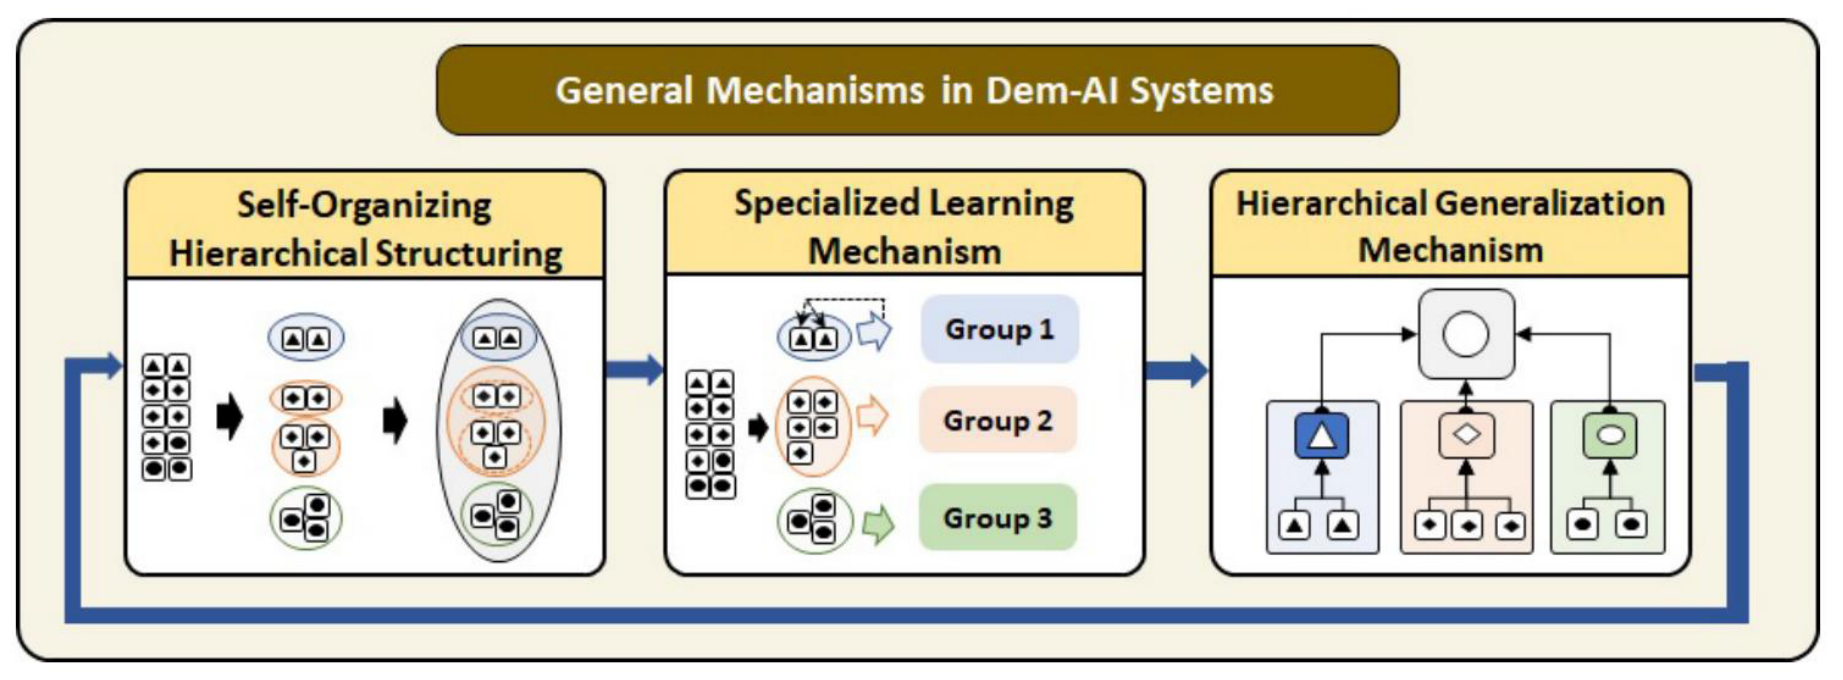
\includegraphics[scale=0.25]{DemIA}

\begin{itemize}

  \item Definizione ed obiettivo\\
  L'apprendimento democratizzato studia processi duali ,accoppiati e operanti insieme, specializzato-generalizzato in una struttura gerarchica auto-organizzante di sistemi di apprendimento distribuiti su larga scala. I processi specializzati e generalizzati devono operare congiuntamente verso un obiettivo di apprendimento finale identificato come l'esecuzione di un apprendimento collettivo da agenti di apprendimento prevenuti, che si impegnano ad apprendere dai propri dati utilizzando le loro limitate capacità di apprendimento. In quanto tale, l'obiettivo finale di apprendimento del sistema Dem-AI è stabilire un meccanismo per risolvere collettivamente compiti di apprendimento complessi comuni (singoli o multipli) da un gran numero di agenti di apprendimento
  \item Processo specializzato\\
  Questo processo viene utilizzato per sfruttare le capacità di apprendimento specializzate degli agenti di apprendimento e dei gruppi specializzati sfruttando i dati raccolti. Incorporando la conoscenza generalizzata dei gruppi di livello superiore creati dal meccanismo di generalizzazione, gli agenti di apprendimento possono aggiornare i parametri del loro modello per ridurre il bias nel loro apprendimento personalizzato.
Pertanto, l'obiettivo di apprendimento personalizzato ha come obiettivi: eseguire un apprendimento specializzato e riutilizzare la conoscenza gerarchica generalizzata disponibile.
  \item Processo generalizzato\\
  Il meccanismo di generalizzazione incoraggia i membri del gruppo a condividere la conoscenza quando svolgono compiti di apprendimento con caratteristiche simili e costruiscono livelli gerarchici di conoscenza generalizzata. La conoscenza gerarchica generalizzata aiuta il sistema Dem-AI a mantenere la capacità di generalizzazione per ridurre il bias degli agenti di apprendimento e affrontare in modo efficiente i cambiamenti ambientali o eseguire nuovi compiti di apprendimento.
  
  \item Struttura gerarchica auto-organizzante\\
  La struttura gerarchica dei gruppi specializzati e le relative conoscenze generalizzate sono costruite e regolate secondo un principio di autoorganizzazione basato sulla somiglianza degli agenti di apprendimento. In particolare, questo principio governa l'unione di piccoli gruppi per formare un gruppo più grande che alla fine migliora le capacità di generalizzazione di tutti i membri. Pertanto, i gruppi specializzati ai livelli più alti nella struttura gerarchica hanno più membri e possono costruire una conoscenza più generalizzata e meno distorta adattandosi più rapidamente ai nuovi ambienti.
  
\item Transizione nel duplice processo specializzato-generalizzato\\
Il processo specializzato diventa sempre più importante rispetto al processo generalizzato durante il periodo di formazione. Di conseguenza, il sistema di apprendimento non solo si evolve per acquisire capacità di specializzazione dai compiti appresi, ma perde anche la capacità di affrontare i cambiamenti ambientali come nuovi agenti di apprendimento e nuovi compiti di apprendimento. Nel frattempo, la struttura gerarchica del sistema Dem-AI è auto-organizzata e si è evoluta da un alto livello di plasticità a un alto livello di stabilità, cioè da gruppi specializzati instabili a gruppi specializzati ben organizzati. La transizione del sistema di apprendimento Dem-AI è illustrata in figura con tre sub-meccanismi iterativi come la generalizzazione, l'apprendimento specializzato e il meccanismo di strutturazione gerarchica. Di conseguenza, la transizione del processo duale specializzato-generalizzato rappresenta le fasi di un tipico quadro di apprendimento democratizzato. In quella transizione, gli agenti di apprendimento sono raggruppati in base alle somiglianze dei loro compiti di apprendimento nella fase iniziale. Quindi, il processo generalizzato aiuta nella costruzione di una conoscenza gerarchica generalizzata per i gruppi specializzati dal basso verso l'alto e incoraggia i membri del gruppo a essere vicini. Nel frattempo, i processi di apprendimento specializzati sfruttano l'apprendimento personalizzato per sfruttare i loro set di dati distorti incorporando la conoscenza di gruppo generalizzata di livello superiore dai gruppi di livello superiore a quelli di livello inferiore.

\end{itemize}

\chapter{Apprendimento democratizzato: Progettazione}\label{ch:chapter2}
In questo elaborato,studiamo un nuovo algoritmo di apprendimento distribuito che consiste in: raggruppamento gerarchico, generalizzazione gerarchica e meccanismi di apprendimento con un compito di apprendimento comune per tutti gli agenti di apprendimento.

\begin{itemize}

\item Meccanismo di raggruppamento gerarchico\\

Per costruire la struttura gerarchica del sistema Dem-AI con gruppi di apprendimento specializzati pertinenti, adottiamo l'algoritmo di clustering gerarchico agglomerativo ovvero l'implementazione del dendrogramma da scikit-learn, basato sulla somiglianza o non somiglianza di tutti gli agenti di apprendimento.
Il metodo del dendrogramma viene utilizzato per esaminare le relazioni di somiglianza tra gli individui ed è spesso utilizzato per l'analisi dei cluster in molti campi di ricerca. Durante l'implementazione, la topologia ad albero del dendrogramma viene costruita unendo le coppie di agenti o cluster che hanno la distanza minore tra loro, seguendo lo schema bottom-up. Di conseguenza, la distanza misurata è considerata come le differenze nelle caratteristiche degli agenti di apprendimento (ad esempio, parametri del modello locale o gradienti della funzione dell'obiettivo di apprendimento). Poiché otteniamo prestazioni simili implementando il clustering basato su parametri o gradienti del modello, in quanto segue presentiamo solo un meccanismo di clustering utilizzando i parametri del modello locale. \\
Dati i parametri del modello locale $\omega_n$ = ($\omega_{n,1}$,..., $\omega_{n,M}$) dell'agente di apprendimento \textsl{n}, dove \textsl{M} è il numero di parametri di apprendimento, la misura della distanza tra due agenti $\phi_{n,l}$ è derivata in base al modello euclideo distanza come $\phi_{n,l}$ =  ||$\omega_n$ - $\omega_l$|| 
Inoltre, consideriamo il metodo del collegamento medio per il calcolo della distanza tra un agente e un cluster utilizzando la distanza euclidea tra i parametri del modello dell'agente e i parametri del modello medio dei membri del cluster.
Di conseguenza, la struttura gerarchica ad albero è sotto forma di un albero binario con molti livelli. Richiederà quindi, costi computazionali e di archiviazione inutilmente elevati per mantenere i dati ed è un modo inefficiente per mantenere un gran numero di modelli generalizzati di basso livello per piccoli gruppi. Di conseguenza, manteniamo solo i K livelli superiori nella struttura ad albero e scartiamo la struttura di livello inferiore. Pertanto, al livello K più alto, il sistema potrebbe avere due grandi gruppi che hanno un gran numero di agenti di apprendimento.


\item Generalizzazione gerarchica e meccanismo di apprendimento\\

La struttura gerarchica di livello K emerge attraverso il clustering agglomerante. Di conseguenza, il sistema costruisce K livelli della generalizzazione, come in Figura. Pertanto, proponiamo problemi di apprendimento generalizzato gerarchico (HGLP) per costruire questi modelli generalizzati per gruppi specializzati in una forma ricorsiva, a partire dalla costruzione del modello globale $w^K$ al livello superiore \textsl{K} come segue. \\
Problema HGLP al livello K. \\
$\min_{W^K}L^K$ = $\sum_{k=1}^N k^2$

\end{itemize}
\chapter{Apprendimento democratizzato: Algoritmo e risultati}\label{ch:chapter4}
Riportiamo di seguito il DemLearn tramite uno pseudocodice.

\begin{algorithm}[H]
 \KwData{K, T, $\tau$}
 \For{t=0,...,T-1}{
 	\For{learning agent n=1,...,N}{
 	L'agente \textsl{n} usa il modello del gruppo superiore $w_{n,t}^{(1)}$ come modello iniziale. L'agente \textsl{n} aggiorna iterativamente il modello di apprendimento personalizzato $w_{(n,t+1)}^{(0)}$ come minimizzatore inesatto,  ovvero basato sul gradiente, del seguente problema: $min_{w\in W}L_n^{(0)}(w|D_n)+\frac{\mu}{2}||w-w_{(n,t)}^{(1)}||^2$ \hspace{1cm} (8) L'agente \textsl{n} invia il modello di apprendimento aggiornato al server.
 	}
 	\If{t mod $\tau$=0} {
 	Il server ricostruisce la struttura gerarchica mediante l'algoritmo di clustering.
 	}
 	Aggiornamento gerarchico: ogni gruppo i ad ogni livello k esegue un aggiornamento per il suo modello di apprendimento dal basso verso l'alto per aggiornare il contributo dei membri del gruppo. $w_{(i,t+1)}^{(k)}=\sum_{j\in S_{(i,k)}}\frac{N_{(g,j)}^{(k-1)}}{N_{(g,i)}^{(k)}}w_{(j,t+1)}^{(k-1)}$\hspace{1cm} (9) Dopo che il modello di livello superiore è stato aggiornato, i livelli inferiori iniziano ad aggiornarsi dall'alto verso il basso per il contributo del gruppo superiore come segue: $w_{(i,t+1)}^{(k)}=\alpha w_{(t+1)}^{(k+1)}+(1-\alpha )w_{(i,t+1)}^{(k)}$ \hspace{1cm} (10) I modelli di apprendimento aggiornati al livello 1 (vale a dire, $w_{(t+1)}^{(1)}$) vengono quindi trasmessi a tutti gli agenti per aggiornare i loro modelli locali seguendo l'equazione (10).}
\caption{Algoritmo democratizzato}
\end{algorithm}
In questo paragrafo, convalidiamo l'efficacia dell'algoritmo DemLearn con MNIST, Fashion-MNIST [21], Set di dati Federated Extended MNIST e CIFAR-10 rispettivamente per il riconoscimento di cifre scritte a mano, immagini di moda e per il riconoscimento di oggetti. Conduciamo gli esperimenti con 50 clienti, in cui ogni cliente ha numeri mediani di campioni di dati a 64, 70 e 785 con MNIST, set di dati Fashion MNIST e CIFAR-10, rispettivamente. Diversamente da questi tre set di dati, sperimentiamo anche il set di dati FE-MNIST che ha un numero maggiore di classi come 10 cifre, 25 minuscole e 25 maiuscole. Di conseguenza, selezioniamo 50 clienti da 3559 utenti che hanno almeno 50 campioni di dati nel set di dati FE-MNIST. Utilizzando questi set di dati, il 20\% dei campioni di dati su ciascun client viene utilizzato per valutare le prestazioni di test del modello. Dividiamo il set di dati totale in modo tale che ogni cliente disponga di una piccola quantità di dati da due etichette specifiche tra i dieci complessivi in entrambi i set di dati. In tal modo, replichiamo uno scenario di set di dati personali distorti, ovvero dati altamente sbilanciati e un numero limitato di campioni di addestramento possono essere raccolti presso gli agenti. I modelli di apprendimento sono costituiti da due livelli di convoluzione seguiti da due livelli di pooling e due livelli completamente connessi, mentre nel set di dati CIFAR-10 vengono utilizzati tre livelli di convoluzione. Impostiamo il periodo di aggiornamento $\tau=1$ e convalidiamo le prestazioni della proposta algoritmo con K = 4 livelli generalizzati. DemLearn, FedAvg e FedProx utilizzano il tasso di apprendimento comune $\eta$ = 0.05, epoca locale E = 2, dimensione batch B = 10.
Per FedProx, impostiamo il parametro $\tau$ = 0,5. Nel frattempo, pFedMe necessita di una messa a punto dettagliata per ottenere un'accuratezza competitiva per diversi set di dati.\\
Gli approcci FL esistenti come FedProx e FedAvg si concentrano maggiormente sulle prestazioni di apprendimento del modello globale piuttosto che sulle prestazioni di apprendimento dei clienti. Pertanto, per le prossime applicazioni personalizzate, implementiamo DemLearn e misuriamo le prestazioni di apprendimento di tutti i clienti e dei modelli di gruppo. In particolare, conduciamo valutazioni per la specializzazione (C-SPE) e la generalizzazione (C-GEN) dei modelli di apprendimento in media presso gli agenti che sono definiti solo come le prestazioni nei loro dati di test locali e i dati di test collettivi di tutti gli agenti nella regione. Di conseguenza, indichiamo Global come prestazione del modello globale; e GGEN e G-SPE sono rispettivamente le prestazioni medie di generalizzazione e specializzazione dei modelli di gruppo. Oltre alle prestazioni C-SPE standard per i modelli locali, le prestazioni C-GEN introdotte sono una metrica importante che mostra le capacità generalizzate dei modelli locali. Anche se i modelli locali distorti possono raggiungere valori C-SPE elevati fin dall'inizio, in particolare a causa dei loro piccoli set di dati locali, hanno ancora capacità generalizzate molto basse che possono aiutare a produrre buone previsioni in base ai frequenti cambiamenti degli utenti. Nel frattempo, i modelli globali e di gruppo hanno le capacità generalizzate più elevate, ma capacità specializzate inferiori durante la distribuzione ai client.\\\\
Nelle figure seguenti sono stati condotti alcuni confronti delle prestazioni con i seguenti metodi, DemLearn con i tre metodi FL, FedAvg, FedProx e pFedMe come linee di base su quattro set di dati di riferimento, MNIST, Fashion MNIST, FE- MNIST e CIFAR-10. Le valutazioni sperimentali mostrano che l'approccio proposto supera le linee di base in termini di velocità di convergenza, in particolare per ottenere migliori prestazioni di generalizzazione del client. Osserviamo che il modello locale richiede solo 40 round per raggiungere il livello di prestazioni C-GEN dell'80\% utilizzando l'algoritmo proposto, mentre gli algoritmi FL esistenti come FedProx, FedAvg e pFedMe impiegano più di 80 round globali per raggiungere un livello quasi competitivo livello di prestazioni come il nostro. Inoltre, dopo 100 round, Dem Learn ottiene prestazioni di generalizzazione del cliente medie migliori (ad esempio, 88,77\%) tra i modelli di client e prestazioni C-SPE  comparabili a partire da FedAvg e pFedMe.\\
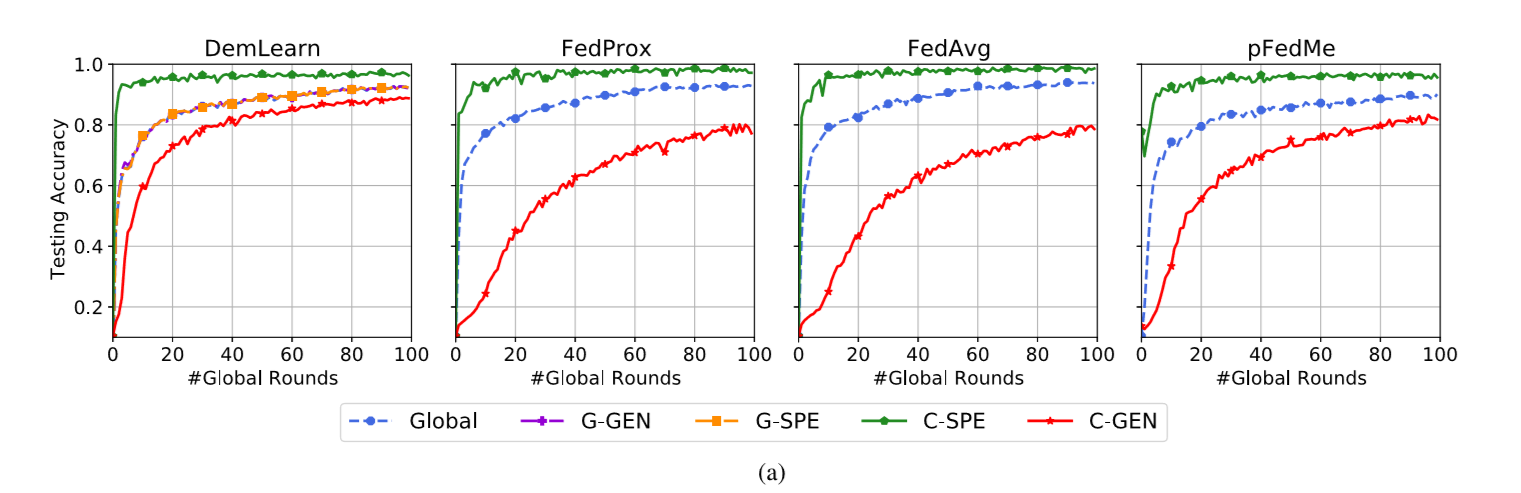
\includegraphics[scale=0.4]{DemLearnMNIST}\\
Notiamo che DemLearn ha prestazioni nettamente superiori con il set di dati MNIST\\\\
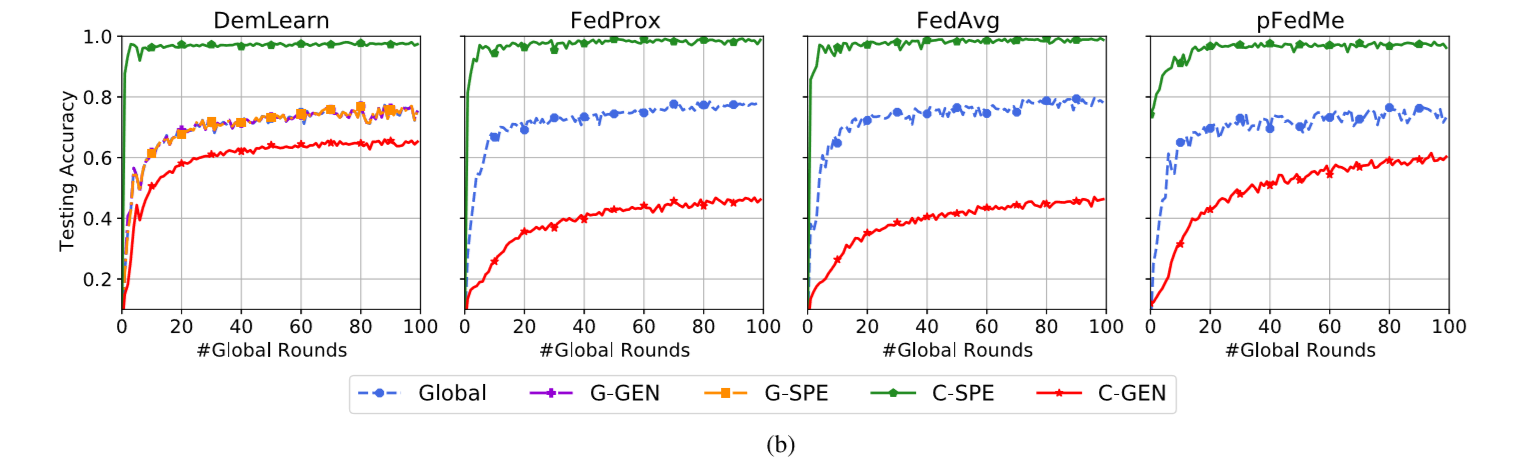
\includegraphics[scale=0.4]{DemLearnFashionMNIST}\\
Anche qui DemLearn è più veloce dei suoi concorrenti con il set dati FashionMNIST\\\\
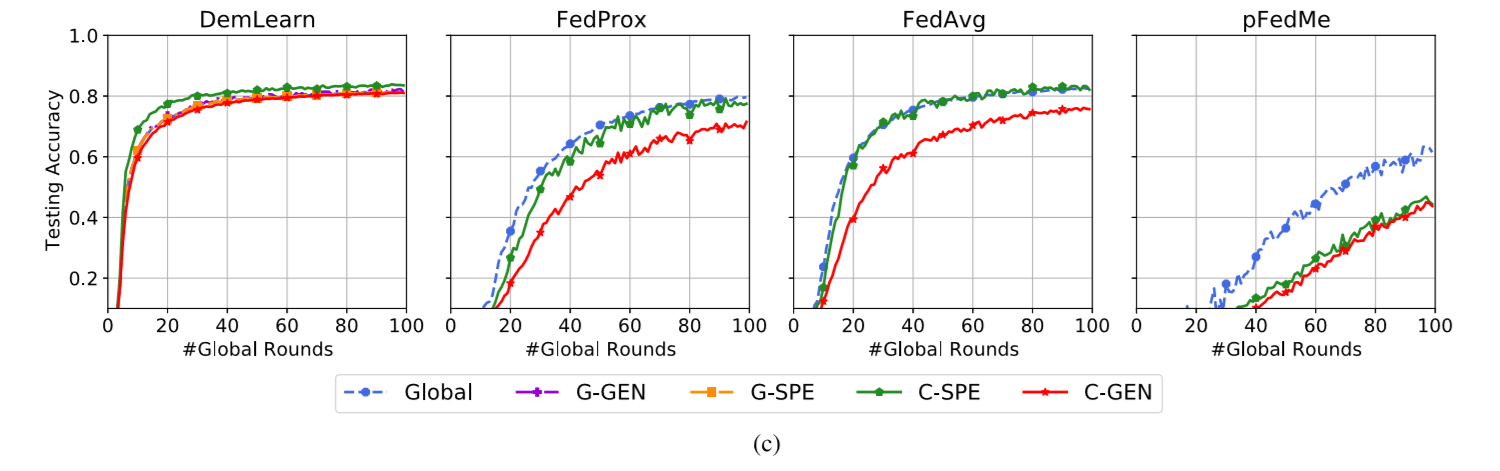
\includegraphics[scale=0.4]{DemLearnFederatedExtMNIST}\\\\
Tutti gli altri algoritmi hanno mostrato prestazioni inferiori e più fluttuanti rispetto a quelle degli altri algoritmi per il set di dati FE-MNIST. pFedMe ottiene un lento miglioramento dei modelli client sia nella specializzazione che nella generalizzazione. Nel frattempo, DemLearn mostra velocità ed efficienza di convergenza stabili per ottenere prestazioni costantemente elevate dei modelli di apprendimento a tutti i livelli.\\\\
\includegraphics[scale=0.5]{cifar10Comparison}\\\\
Osserviamo che DemLearn subisce un leggero degrado delle prestazioni C-SPE e Global per ottenere prestazioni C-GEN elevate. Dopo 100 round, DemLearn dimostra buone capacità di apprendimento di compromesso dei modelli client con C-SPE elevato (79,09\%) prestazioni C-GEN (57\%) e mentre altri algoritmi di base producono solo modelli locali distorti con capacità generalizzate basse.\\\\
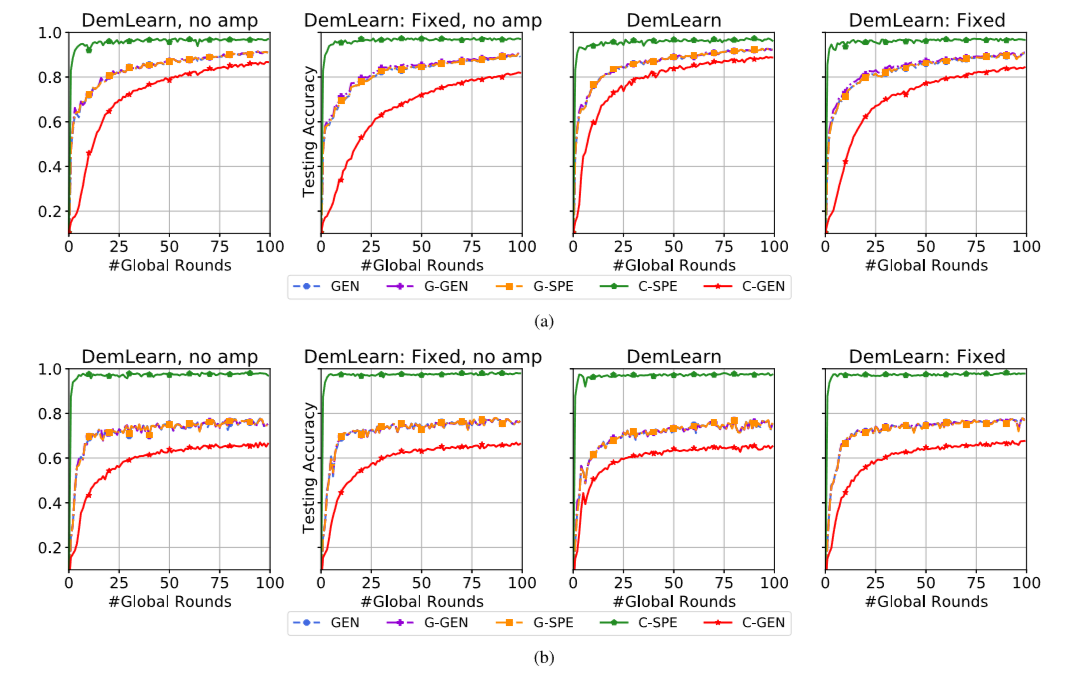
\includegraphics[scale=0.5]{AlgoStructureComp}
Valutiamo e confrontiamo le prestazioni dell'algoritmo proposto per una struttura gerarchica fissa e auto-organizzante attraverso la ricostruzione periodica (cioè, $\tau=1$). Osserviamo che DemLearn beneficia del meccanismo di autoorganizzazione e può fornire una capacità di generalizzazione leggermente migliore dei modelli client. Inoltre, l'amplificazione nei primi cinque cicli aiuta l'algoritmo proposto a velocizzare le prestazioni iniziali dell'algoritmo DemLearn.\\
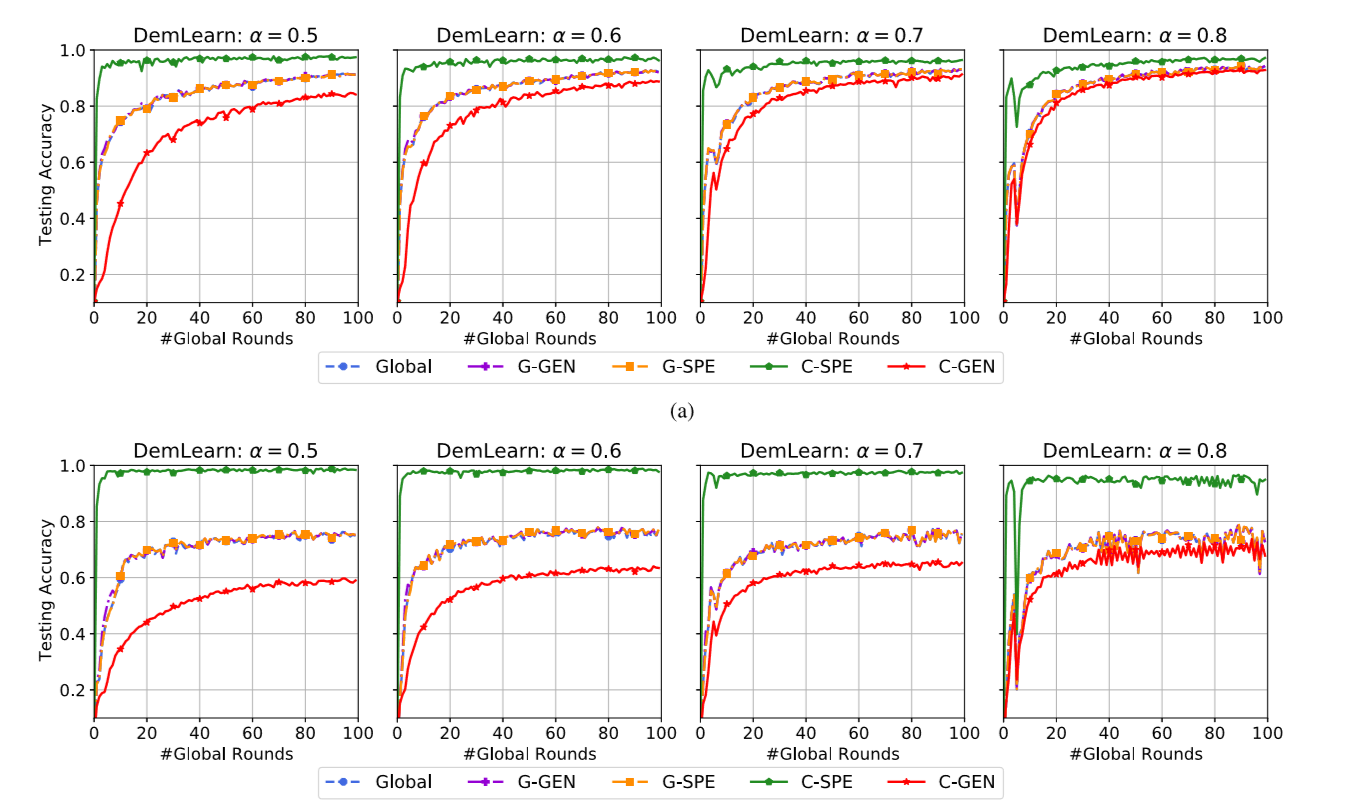
\includegraphics[scale=0.4]{DemAlpha}\\
Mostriamo adesso l'impatto del parametro $\alpha$ nell'accuratezza del test dei set di dati MNIST e Fashion-MNIST, come mostrato. Come si può vedere nei risultati, quando $\alpha$ è grande, otteniamo prestazioni elevate del cliente generalizzazione mentre un leggero degrado nelle loro capacità specializzate.
Pertanto, l'aumento del valore di $\alpha$ migliora la generalizzazione, ma riduce anche in misura marginale le prestazioni di specializzazione dei modelli client. Poiché $\alpha=\mu_{k+1}/(\mu_k+\mu_{k+1})$ controlla il contributo dei modelli di apprendimento del gruppo superiore e dei membri del gruppo, la modifica di $\alpha$ produce l'impatto sulla diffusione della conoscenza generalizzata dai gruppi superiori ai gruppi e ai clienti di livello inferiore. Ad ogni livello k, il valore più alto di $\alpha$ indica che l'obiettivo è più focalizzato sulla minimizzazione del divario con il modello del gruppo superiore a k + 1 rispetto ai modelli del gruppo inferiore a k - 1. Inoltre, valutiamo l'impatto di altri parametri , come $\mu$, K, $\tau$ ma non mostrano effetti evidenti sulle prestazioni di DemLearn probabilmente a causa delle impostazioni di simulazione su piccola scala. Oltre a ciò, ridurre la frequenza degli aggiornamenti del cluster aumentando il parametro $\tau$ può aiutare l'algoritmo a ottenere prestazioni comparabili con un minor costo di riorganizzazione della struttura gerarchica. Tuttavia, a causa della portata limitata dei set di dati e delle impostazioni simulati, si crede che l'impatto dei parametri definiti sulle prestazioni dell'algoritmo proposto si realizzi meglio quando si valuta l'algoritmo con dati più pratici e sperimentali.\\
Oltre alla distanza euclidea tra i parametri di apprendimento nell'algoritmo di clustering gerarchico, possiamo anche valutare la distanza $\phi_{n,t}^{(cos)}$ tra due modelli di apprendimento tramite la somiglianza del coseno con segue:\\
\\ $\phi_{n,t}^{(cos)}=cos(w_n,w_l)=\frac{\sum_{m=1}^M w_{n,m}w_{l,m}}{\sqrt{\sum_{m=1}^M}w_{n,m}^2\sqrt{\sum_{m=1}^M}w_{l,m}^2}$ \hspace{1cm} (11)\\
I risultati sperimentali dimostrano che i modelli client e di gruppo mostrano prestazioni di apprendimento quasi simili e diverse tendenze della topologia del cluster utilizzando l'algoritmo DemLearn. Come mostrato nel Client-GEN, alcuni valori anomali contribuiscono al calo delle prestazioni client-GEN durante la formazione. Allo stesso tempo, la maggior parte dei clienti ha capacità generalizzate paragonabili al modello globale. Di conseguenza, l'illustrazione ci aiuta ulteriormente a capire i clienti estremamente diversi con prestazioni C-GEN basse. Ciò significa che, in ogni round, i valori anomali vengono rilevati (e classificati) da un meccanismo di raggruppamento che è estremamente diverso da altri parametri del modello client. Tuttavia, notiamo che i valori anomali non sono sempre gli stessi e cambiano durante gli aggiornamenti del modello locale. Ma alcuni appaiono più volte e forniscono informazioni significative per il sistema di apprendimento. Inoltre la differenza nella topologia del cluster non influisce molto sulle prestazioni di apprendimento complessive.\\
Rispetto a FedAvg e FedProx, abbiamo un costo computazionale sul dispositivo simile per risolvere il problema PLP utilizzando il metodo di discesa del gradiente. Diversamente dagli altri, pFedMe richiede passaggi aggiuntivi per l'approssimazione $\theta$ e quindi richiede più tempo di calcolo sul dispositivo client. D'altra parte, per il tempo di calcolo richiesto sul server, l'algoritmo DemLearn richiede un costo di calcolo aggiuntivo per il clustering gerarchico e un costo trascurabile per gli aggiornamenti gerarchici. Notiamo che il costo del clustering gerarchico dipende dalla dimensione del modello e dal numero di agenti di apprendimento. In linea di principio, l'algoritmo standard per il clustering gerarchico agglomerativo ha una complessità temporale di O(n3) e richiede una memoria O(n2) [24].Valutiamo l'algoritmo con n = 50 utenti e otteniamo in media un tempo di esecuzione di 0,0015 secondi per passo quando si utilizza un computer con CPU i7-7700K e una memoria di 32 GB. Per il costo di comunicazione, tutti gli algoritmi richiedono costi simili per inviare i parametri del modello.\\\\
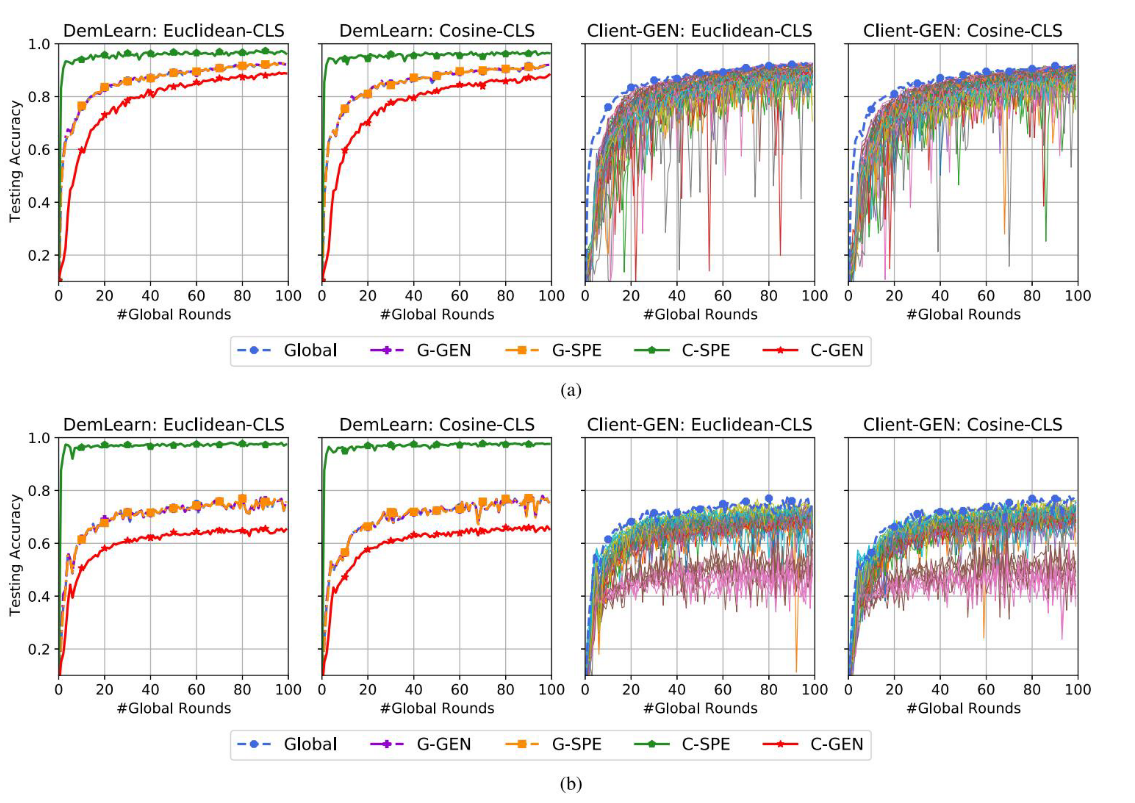
\includegraphics[scale=0.4]{ClusteringLast}\\\\
In pratica, per implementare una tipica struttura gerarchica, i sistemi Dem-AI possono includere tre entità. Un server cloud che gestisce il modello globale (nodo radice) e i suoi gruppi generalizzati di sottolivello. Server regionali distribuiti, che sono server perimetrali distribuiti all'interno di ciascuna regione e il cui ruolo è gestire i sottogruppi e gli agenti di apprendimento e agenti di apprendimento.
Purtroppo l'implementazione per il clustering gerarchico è centralizzata in questi esperimenti. Tuttavia, il meccanismo di clustering gerarchico agglomerante unisce gli agenti e i gruppi di apprendimento dal basso verso l'alto, e quindi è possibile implementarlo in modo decentralizzato. Pertanto, possiamo gestire il clustering gerarchico nel server cloud per i livelli superiori e l'implementazione decentralizzata per le regioni nei server perimetrali per i gruppi di livello inferiore. Inoltre, questo meccanismo di raggruppamento può mitigare gli effetti negativi dell'aggregazione di agenti di apprendimento estremamente diversi per costruire modelli gerarchici generalizzati. In questo modo, manteniamo tre o più livelli di modelli generalizzati invece di un unico modello globale. Per quanto ne sappiamo, questo design non è stato ancora preso in considerazione in recenti studi sul FL personalizzato.
\chapter{Conclusioni}\label{ch:conclusioni}
La nuova filosofia Dem-AI ha fornito linee guida generali per meccanismi di strutturazione gerarchica specializzati, generalizzati e auto-organizzanti in sistemi di machine learning distribuiti su larga scala. Ispirati da queste linee guida, abbiamo formulato i problemi gerarchici di apprendimento generalizzato e sviluppato un nuovo algoritmo di apprendimento distribuito, DemLearn. In questo lavoro, basato sulla somiglianza nelle caratteristiche di apprendimento, il clustering agglomerativo consente l'auto-organizzazione degli agenti di apprendimento in una struttura gerarchica, che viene aggiornata periodicamente. L'analisi dettagliata delle valutazioni sperimentali ha mostrato i vantaggi e gli svantaggi dell'algoritmo proposto. Rispetto al FL convenzionale, mostriamo che DemLearn in modo significativo migliora le prestazioni di generalizzazione dei modelli client senza compromettere in gran parte le prestazioni di specializzazione dei modelli client. Di conseguenza, DemLearn consente buone capacità di apprendimento del compromesso dei modelli client con prestazioni C-SPE e C-GEN elevate, mentre altri algoritmi possono produrre solo modelli locali distorti con capacità generalizzate basse. Queste osservazioni favoriscono una migliore comprensione e un miglioramento delle prestazioni di specializzazione e generalizzazione dei modelli di apprendimento nei futuri sistemi Dem-AI. L'apprendimento democratizzato fornisce ingredienti unici per sviluppare futuri sistemi intelligenti personalizzati distribuiti.
A tal fine, il progetto di apprendimento potrebbe essere ulteriormente studiato con set di dati personalizzati, esteso per capacità di apprendimento multi-task e convalidato con una generalizzazione effettiva per i nuovi utenti e cambiamenti ambientali. Trasformando in realtà i sistemi generali di apprendimento distribuito, il Dem-AI deve essere analizzato in profondità da una varietà di prospettive come la robustezza e la diversità dei modelli di apprendimento e i nuovi meccanismi di trasferimento e distillazione della conoscenza. Inoltre, è possibile incorporare il design flessibile con approcci attuali come meta-learning e metodi basati sull'ottimizzazione per migliorare ulteriormente la personalizzazione in FL.
\chapter{Bibliografia}\label{ch:biblio}
\begin{enumerate}
 \item Self-organizing Democratized Learning: Towards Large-scale Distributed Learning Systems, Minh N. H. Nguyen, Shashi Raj Pandey, Tri Nguyen Dang, Eui-Nam Huh, Nguyen H. Tran, Walid Saad, Choong Seon Hong
 \item Zhou, Zhi-Hua. Machine learning. Springer Nature, 2021.
 \item Samek, Wojciech, et al., eds. Explainable AI: interpreting, explaining and visualizing deep learning. Vol. 11700. Springer Nature, 2019.
 \item Li, Li, et al. "A review of applications in federated learning." Computers $\&$ Industrial Engineering 149 (2020): 106854.
\end{enumerate}
\addcontentsline{toc}{chapter}{Bibliografia}
\bibliographystyle{plain}
\bibliographystyle{unsrt}
%\bibliography{sp,xml}

\end{document} 